\vspace{-0.5cm}
\section{Introduction}
\label{sec:intro}
\vspace{-0.15cm}


% 11/10 v4
Diffusion Models (DMs) have emerged as a powerful class of generative models, demonstrating state-of-the-art performance in tasks such as image synthesis \cite{ho2020denoisingdiffusionprobabilisticmodels,song2020generativemodelingestimatinggradients,song2021scorebasedgenerativemodelingstochastic,song2022denoisingdiffusionimplicitmodels,rombach2022high,podell2023sdxlimprovinglatentdiffusion,lin2023magic3dhighresolutiontextto3dcontent} conditional generation \cite{Avrahami_2022,meng2022sdeditguidedimagesynthesis,mou2023t2iadapterlearningadaptersdig,bartal2023multidiffusionfusingdiffusionpaths,bashkirova2023masksketchunpairedstructureguidedmasked,huang2023composercreativecontrollableimage,zhang2023addingconditionalcontroltexttoimage,ni2023conditional,podell2023sdxlimprovinglatentdiffusion}, and precise image editing \cite{mokady2023null,miyake2023negative,wallace2023edict,han2024proxedit,garibi2024renoise,huberman2024edit}. Unlike GANs, which rely on adversarial training to generate samples \cite{goodfellow2014generativeadversarialnetworks,metz2016unrolled,gulrajani2017improved,arjovsky2017towards,karras2018progressivegrowinggansimproved,brock2019largescalegantraining,karras2019stylebasedgeneratorarchitecturegenerative,karras2020traininggenerativeadversarialnetworks,Karras2021}, diffusion models (DMs) use a stochastic process that incrementally adds Gaussian noise to data, then reverses this process to generate new samples. This iterative approach, while computationally intensive, enables greater control over sample quality and diversity through guided sampling methods \cite{ho2022classifier,dieleman2022guidance,ho2022imagenvideohighdefinition,Meng_2023_CVPR,karras2024guiding}. In contrast, GANs often suffer from mode collapse \cite{gulrajani2017improved,arjovsky2017towards,metz2016unrolled}, which hinders output diversity and training stability. Diffusion-based algorithms can thus offer a key advantage by balancing quality-diversity tradeoffs, frequently achieved with Classifier-free Guidance (CFG) \cite{ho2022classifier}. Both the role of diffusion noise scheduling and the network's convergence properties are essential for improving performance and applicability \cite{karras2022elucidating,lu2022dpmsolverfastodesolver,lu2023dpmsolverfastsolverguided,zheng2023dpm,karras2024analyzingimprovingtrainingdynamics,salimans2022progressivedistillationfastsampling,park2024textitjumpstepsoptimizingsampling,karras2024guidingdiffusionmodelbad}. 

Consistency Models (CMs), designed to accelerate the diffusion process, provide a more efficient alternative by reducing the number of function evaluations (NFE) needed for generation \cite{song2023consistency,kim2023consistency,kim2024generalized,li2024bidirectional,heek2024multistep,lu2024simplifyingstabilizingscalingcontinuoustime,lee2025truncatedconsistencymodels}. These models achieve this by aligning data points along the Probability-flow (PF) ODE of the stochastic forward process, using either consistency distillation (CD) or consistency training (CT) \cite{song2023consistency}. While CD models have been widely applied in real-time image synthesis and fast editing via distillation \cite{luo2023latent,starodubcev2024invertible}, the development of CT models remain relatively unexplored. This is primarily because CT, as a fully self-supervised and data-driven approach, requires a well-crafted training curriculum to be trained successfully ~\cite{song2023improved,ect}.

\begin{figure}[t!]
    \centering
    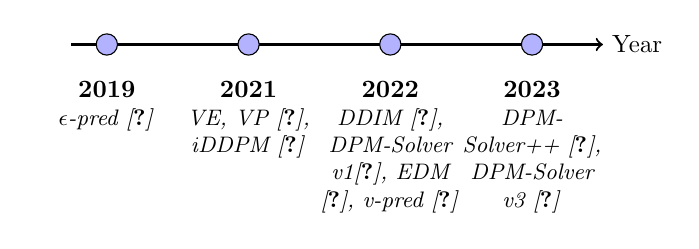
\begin{tikzpicture}[scale=0.9, transform shape]
        % Horizontal timeline line
        \draw[thick, ->] (0, 0) -- (7.5, 0) node[right] {Year};

        % Timeline events with captions
        % Event 1
        \draw[fill=blue!30] (0.5, 0) circle (0.15) node[below=0.4cm] {\parbox{2cm}{\centering \textbf{2019} \\ \small\textit{$\epsilon$-pred \cite{ho2020denoisingdiffusionprobabilisticmodels}}}};

        % 2021
        \draw[fill=blue!30] (2.5, 0) circle (0.15) node[below=0.4cm] {\parbox{2cm}{\centering \textbf{2021} \\ \small\textit{VE, VP \cite{song2021scorebasedgenerativemodelingstochastic}, iDDPM \cite{nichol2021improveddenoisingdiffusionprobabilistic} }}};

        % 2022
        \draw[fill=blue!30] (4.5, 0) circle (0.15) node[below=0.4cm] {\parbox{2cm}{\centering \textbf{2022} \\ \small\textit{DDIM \cite{song2022denoisingdiffusionimplicitmodels}, DPM-Solver v1\cite{lu2022dpmsolverfastodesolver}, EDM \cite{karras2022elucidating}, v-pred \cite{salimans2022progressivedistillationfastsampling}}}};

        % 2023
        \draw[fill=blue!30] (6.5, 0) circle (0.15) node[below=0.4cm] {\parbox{2cm}{\centering \textbf{2023} \\ \small\textit{DPM-Solver++ \cite{lu2023dpmsolverfastsolverguided}, DPM-Solver v3 \cite{lu2023dpmsolverfastsolverguided} }}};

    \end{tikzpicture}
    
    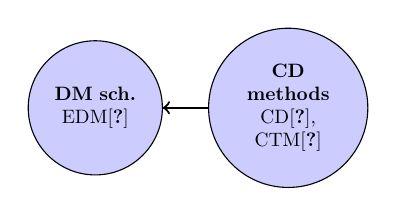
\begin{tikzpicture}[scale=0.7, transform shape]
        \node[draw, circle, fill=blue!20, minimum size=1.2cm, text width=2cm, align=center] (A) at (0, 0) {\textbf{DM sch.} EDM\cite{karras2022elucidating}};

        \node[draw, circle, fill=blue!20, minimum size=1.2cm, text width=2cm, align=center] (B) at (3.5, 0) {\textbf{CD methods} CD\cite{song2023consistency}, CTM\cite{kim2023consistency}};

        \draw[->, thick] (B) -- (A);

        %\node[draw, circle, fill=blue!20, minimum size=1.2cm, text width=2cm, align=center] (C) at (0, 3.5) {\textbf{DM sch.}  $\epsilon$-pred \cite{ho2020denoisingdiffusionprobabilisticmodels} };

        %\node[draw, circle, fill=blue!20, minimum size=1.2cm, text width=2cm, align=center] (D) at (3.5, 3.5) {\textbf{CD methods} LCM\cite{luo2023latent}, TCD\cite{zheng2024trajectoryconsistencydistillationimproved}};

        %\draw[->, thick] (D) -- (C);

    \end{tikzpicture}
    \vspace{-1em}
    \caption{Timeline of key developments in diffusion training/sampling schedulers (top). The schedulers used by pretrained DMs that CD depends on (bottom). The fields of DM and CT are advancing rapidly in multiple directions, and tightly coupling CM with DM would slow down progress. To train a CM under a particular diffusion scheduler, CD-based CMs rely on a teacher DM trained under the same setting, while \textbf{CT is free of such constraint}.} 
    \vspace{-1.5em}
    \label{fig:dm&cd}
\end{figure}


CT, however, offers distinct advantages. First, unlike CD, CT can be trained with any underlying diffusion schedulers. The design space for DM training, sampling, and preconditioning \cite{karras2022elucidating} is an ongoing area of research that has attracted researchers interest ever since the diffusion surge. Therefore, CT's flexibility to train with improved designs makes it more attractive than CD by dropping the dependence of a state-of-the-art DM. An improved diffusion scheduler can be directly utilized in CT, while CD depends on the existence of a DM (Fig.~\ref{fig:dm&cd}). Second, recent studies show that CT, when improved with advanced training techniques, outperforms CD in image generation on FID metrics \cite{song2023improved,ect}. This underscores its potential to surpass CD in both efficiency and quality, making CT as a promising alternative for advancing fast generative modeling. 

Our study fills the missing piece in establishing a comprehensive theory for CT, a data-driven approach for \textit{guidance learning} in 1-step/few-step image generation. We present \textbf{\textit{Invertible Guided Consistency Training}} (iGCT), a novel framework that enables CMs to perform guided generation without requiring DM distillation at training. In training, iGCT decouples the target clean sample from the source to capture effects of both unconditional and conditional noise. For invertibility, iGCT incorporates an independent component, the noiser, which maps images to noise in a single step. This same-dimensional noise, termed as \textit{noise latent} in our paper, serves as a deterministic representation of the input image. Removing the dependency on a teacher DM, iGCT provides greater flexibility and efficiency by eliminating the need of a two-stage training procedure. We show that guidance learned via iGCT removes the high-contrast artifacts (Figs.~\ref{fig:teaser_horse_explain_v2} and \ref{fig:1d_cfg_igct}), a well-known \textit{limitation} observed for CFG trained DMs \cite{ho2022imagenvideohighdefinition,saharia2022photorealistictexttoimagediffusionmodels,bradley2024classifierfreeguidancepredictorcorrector,kynkaanniemi2024applying,karras2024guiding}. Consequently, iGCT achieves higher FID's and Precision/Recall under guided generation compared to multi-step DMs and their distilled CM counterparts. In line with the parallel work on few-step image editing from iCD \cite{starodubcev2024invertible}, we demonstrate that iGCT is effective for 1-step image editing. Following common editing frameworks that applies high guidance after DDIM inversion \cite{mokady2023null,miyake2023negative,han2024proxedit,starodubcev2024invertible}, iGCT is able to match the target class semantics while preserving features inversed from the source image. To summarize, our contributions are as follows:
\begin{itemize}
    \vspace{-0.5em}
    \item We introduce \textbf{\textit{invertible Guided Consistency Training}} (iGCT), a DM independent approach that incorporates guidance into CMs (Sec. \ref{sec:method} and Appendix \ref{appendix:iGCT}). 
    \vspace{-0.5em}
    \item We demonstrate iGCT's ability to trade-off diversity for precision as guidance strength increases, beating CFG trained DMs and distilled CMs by eliminating saturated artifacts under high guidance scale (Figs. \ref{fig:results_guidance} and  \ref{fig:results_fid_prec_rec}).
    \vspace{-0.5em}
    \item We present iGCT’s invertibility, a disjoint contribution that enables efficient inversion and generation using class conditioning, offering a promising framework for real-time image editing (Sec. \ref{sec:image-editing}).
\end{itemize}

